\chapter{Android Application Software}
In order to receive, store, visualize and export the measured data generated by the system, an Android application has been developed.

\section{User Interface}
The application software was developed using an experience-driven model. The main objective regarding the user interface design was to build an app that does what the user expects. The functional logic has been designed to suit the user interface requirements. Experience-driven development lays a strong focus on the recognizability of user interface elements, which in turn means the app design mostly reuses design principles commonly used on the Android Platform. In order to reduce avoidable effort in design, it was decided to standardize the app on Material Design (see \cite{Material}). Material design is the native design guideline for Android versions newer than Lollipop (5.0) and also well-known on older devices, as many apps (including the Google apps) use material design also on older devices. The app tries to follow the Material Design Guidelines as close as possible in order to provide a familiar design to Android users. Most design elements are provided by the Application Support Library (see \cite{AppCompat}) which provides Material design components to old Android Versions back to Gingerbread (API 9).

\begin{figure}[ht]
	\centering
	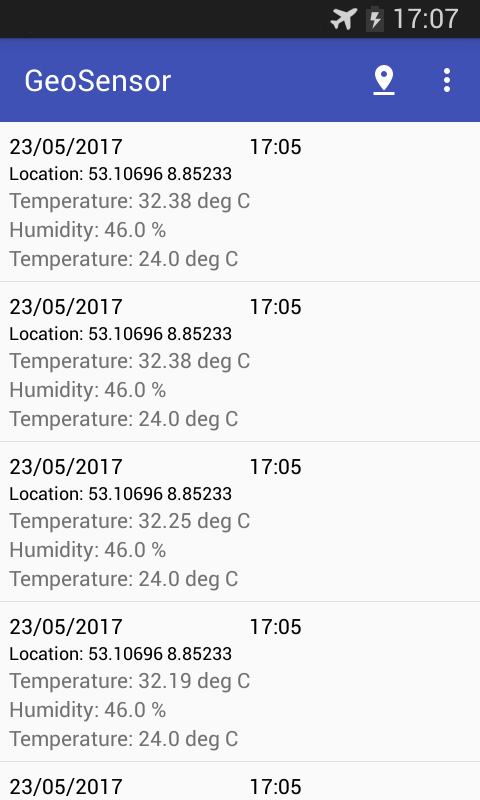
\includegraphics[width=6cm]{src/main_list}
	\caption[Main List]
	{The user interface of the main activity of the app as seen on a Samsung Android 4.2.2 device}
\end{figure}

\subsection{Internationalization}
As not every user feels comfortable using application software in foreign languages, the application is built to fully support localization leveraging the Android resource framework. The applications default language was chosen to be English (stylized as United States) as this is the fallback language international users normally expect in case there is no translation for their language. As a proof of concept and to be used by German-speaking users the app contains a full (meaning the user will not see any text in the default language) German (without further distinction by country) translation. As all user interface elements that might need a translation are included in the R.string resources, the app is prepared for further translations that might be added later. The app design includes the necessary preparations for right-to-left languages, but the compatibility for those languages is not a specific design target that. 

\begin{figure}
\centering
\begin{minipage}{.5\textwidth}
  \centering
  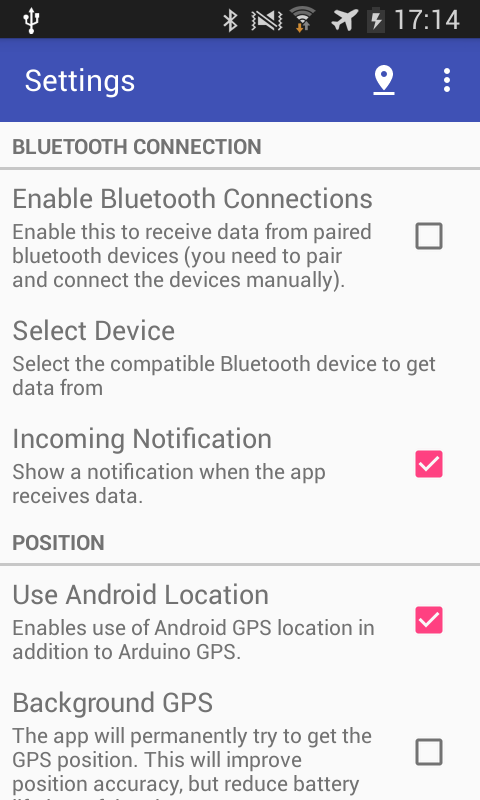
\includegraphics[width=.8\linewidth]{src/settings_en_1.png}
\end{minipage}%
\begin{minipage}{.5\textwidth}
  \centering
  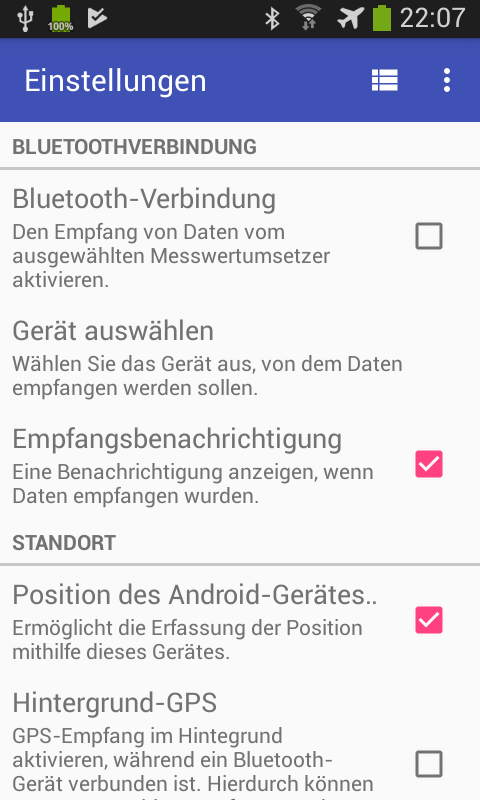
\includegraphics[width=.8\linewidth]{src/settings_de.png}
\end{minipage}
  \caption{Comparison of settings activity in the EN-US and DE-DE locales}
  \label{fig:settings_comp}
\end{figure}

In order to show the types of sensors in the user interface language, the app contains a mechanism to translate the measurement category to the user interface language. The mechanism uses a string array located in the resources to look up the localized denomination. If there is no translation defined, the measurement category is shown as it was transmitted by the transducer.

Times are always shown in the time zone the user has set the device to and formatted according to the local format given by the Android framework. An example of time formatting and sensor type translation can be seen in figure \ref{fig:lang_comp}.

\begin{figure}
\centering
\begin{minipage}{.3\textwidth}
  \centering
  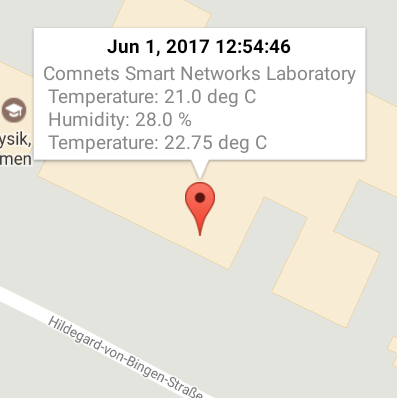
\includegraphics[width=.8\linewidth]{src/marker_en.png}
\end{minipage}%
\begin{minipage}{.3\textwidth}
  \centering
  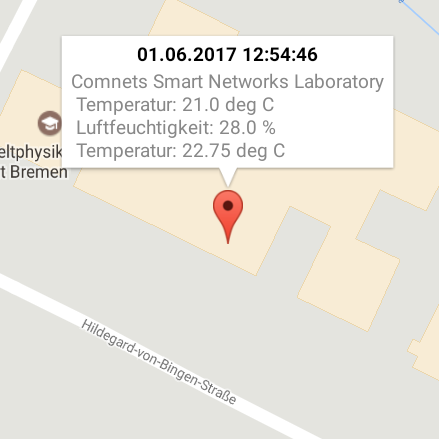
\includegraphics[width=.8\linewidth]{src/marker_de.png}
\end{minipage}
\begin{minipage}{.3\textwidth}
  \centering
  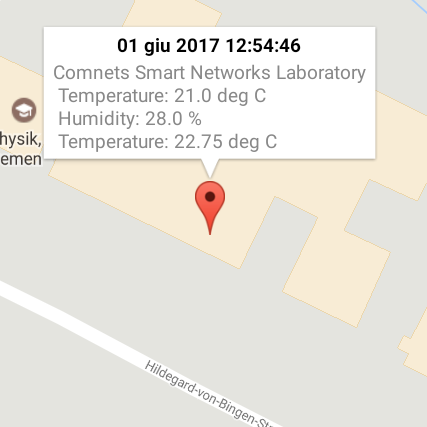
\includegraphics[width=.8\linewidth]{src/marker_it.png}
\end{minipage}
  \caption{Comparison of map marker contents in the en\textunderscore US, de\textunderscore DE and it\textunderscore SM locales.}
  \label{fig:lang_comp}
\end{figure}

\subsection{Toolbar}
Most Android apps use some kind of bar near the top of the screen to allow users to find the basic user interface elements. Often this bar is an \texttt{ActionBar} as provided by the Android framework. As this app is build using the Application Support Library the Toolbar provided by that library is used. The Toolbar contains the control elements needed in the specific Activity and changes accordingly. In most activities (if they are not designed to be modal) there is an overflow menu that contains any element overflowing from the Toolbar and the application settings. The material design guidelines specify that the application settings should always be shown in the overflow menu even if there would be enough space left for a button in the Toolbar itself.

\subsubsection{Export}
\label{subsubs:export}
In order to further process the data acquired by the system, the data can be exported. Even though the data model is object-oriented and contains lists of data which have variable length (the app does not have a priori knowledge of the sensors), the data export feature generates a comma separated values file (.csv-file) including the data acquired from the measurements. The table has a variable width as its width is adjusted to fit the number of sensors and the number of location objects associated with the measurements. The export can be configured to use decimal separators (period \/ full stop or comma) and field separators (comma, semicolon or tab stop) as needed. This setting is exposed in the application settings. Another option included in the application settings is to export only the best location associated with the data record which will make the structure of the exported file more regular as the first sensor will then always be found in the same column. The export however does not assert that the sensors will be exported in a specific order, which means in some cases the data will need to be ordered by an importing application (e.g. using the Excel LOOKUP function analyzing the imported data). The order of the exported sensors should however be consistent for the same transducer configuration. On large data sets the export might take some time, however the user can continue to use the app until the exported data is ready.

Old Android versions allow the App to directly write the export data to the so-called external storage on the Android device. When the export is finished, the app shows an alert containing the path (which is inside a folder called GeoSensor in the external storage root folder) of the exported file. The filenames of the exported file contain an export timestamp. Other apps or a USB connection can be used to open or move the file from the aforementioned folder.

\begin{figure}
\centering
\begin{minipage}{.5\textwidth}
  \centering
  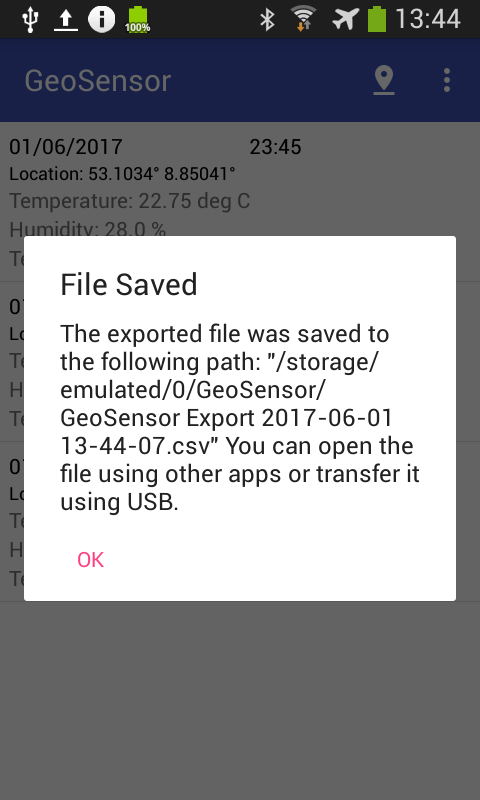
\includegraphics[width=.8\linewidth]{src/export_old.png}
\end{minipage}%
\begin{minipage}{.5\textwidth}
  \centering
  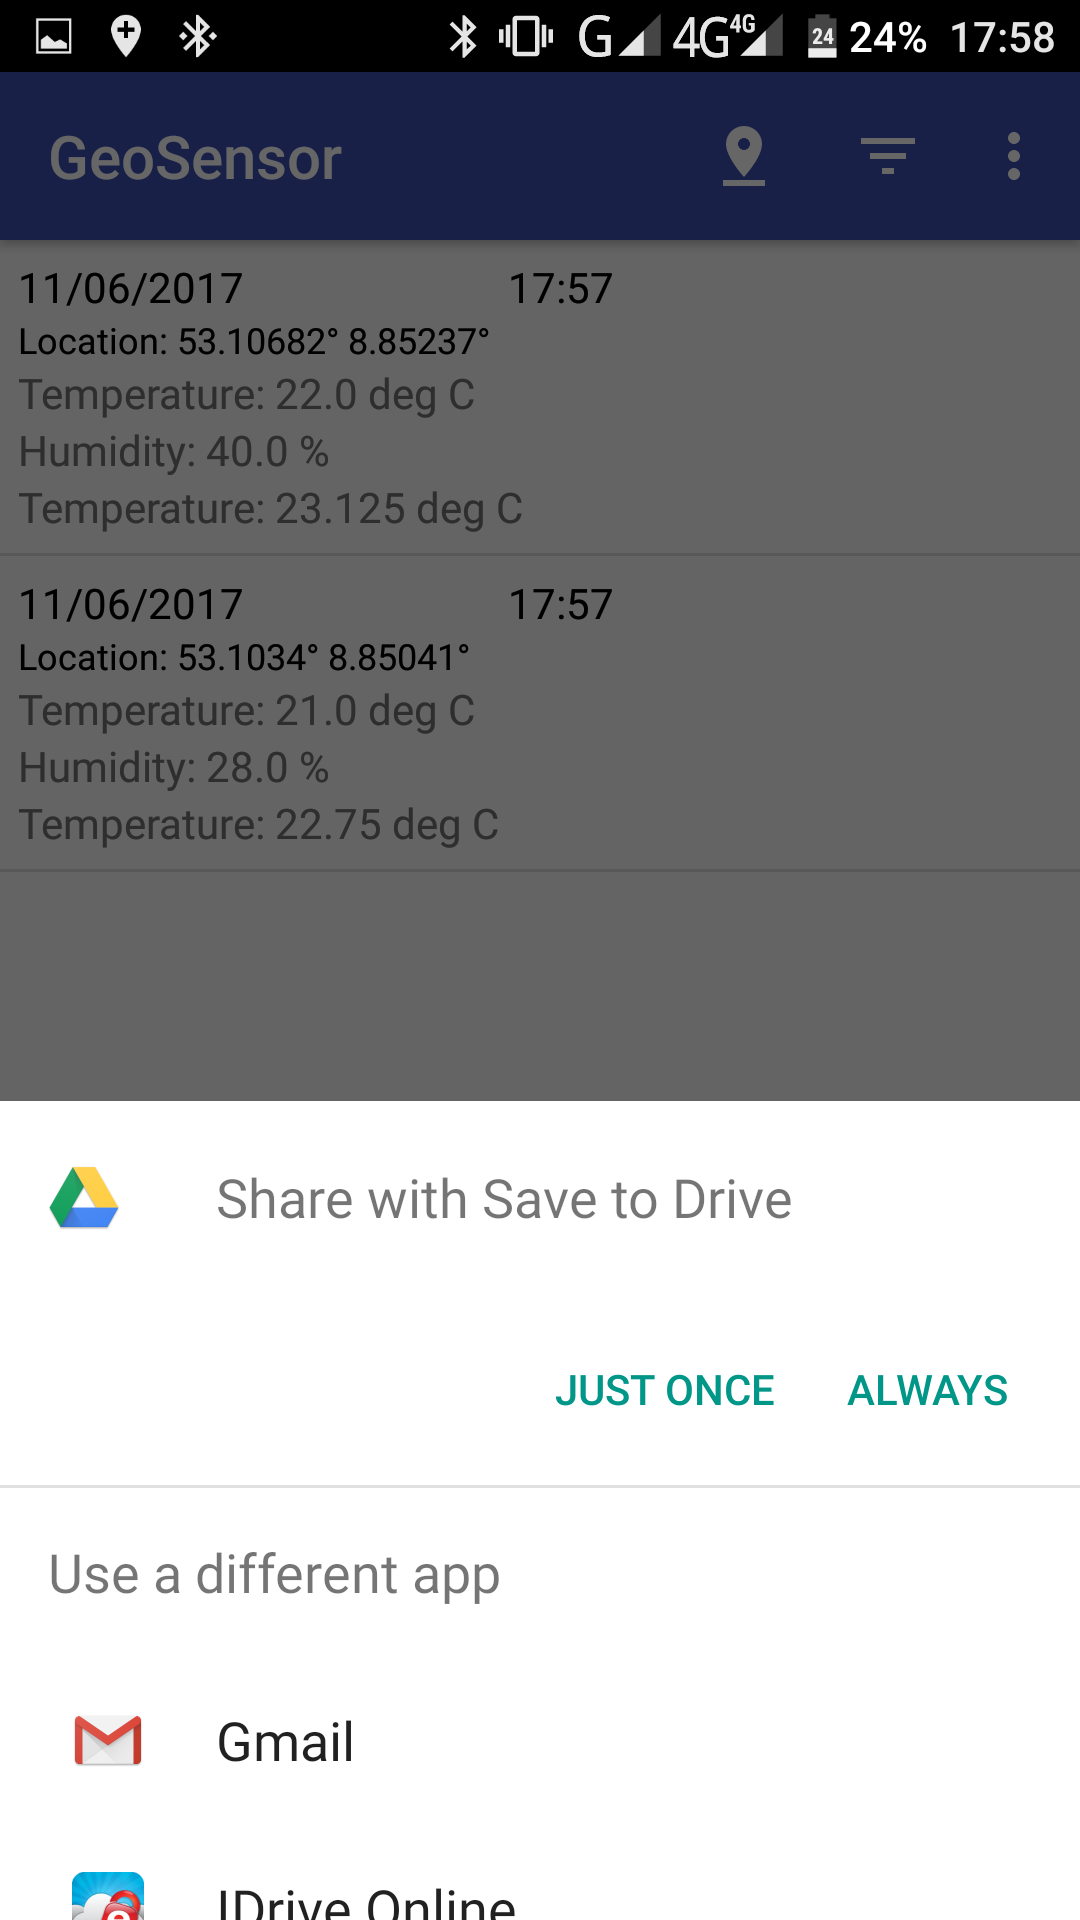
\includegraphics[width=.8\linewidth]{src/export_new.png}
\end{minipage}
\caption{Exporting data in older and newer Android versions}
\label{fig:export_old}
\end{figure}

\paragraph{Export after Android KitKat (4.4)}
In more recent Android versions the file handling works differently. After the data has been prepared, it is exported to an app that can handle general files which mostly includes cloud storage providers. The user is shown a system dialog asking him to choose the app to export the data to. In the dialog, there is a possibility to make the system open the app in the future again without asking. The app used for testing purposes is Google Drive as it is the most widespread cloud storage app in the Android ecosystem.

\subsubsection{Filtering}
\label{subs:filter-ui}
\paragraph{Filter by Time}
The time filter allows to choose a start and end time for the data records shown. The base time used for filtering is the receive time as that is guaranteed to be unique for each measurement data record and it exists for each data record. As the filter is set globally for the whole application, it applies to all views and also to exports. The setting however is not preserved across the application lifecycle which means it is reset when the application is closed. The filter logo changes to the accent color while a filter is deployed.

\subsection{First Start}
When the application is first started, the user is prompted to select a Bluetooth device the app should connect to. Note that as the app uses Googles auto backup feature where available, the application settings might be restored from a previous install if the app is reinstalled on the same device again or in case a backup was transferred to a new device. 

\subsection{Main List}
The main list is the entry point into the application. It is the main activity started first when the app is started. The main list contains a list element for each data record received from the database after applying the filter (see \ref{subs:filter-ui} and \ref{subsubs:filter-tech}). The element shows the receive time and date, the geographic coordinates and the measured values received. When the entry is touched, the details view (see \ref{subs:details-view}) is opened for the data record. When a new data record is received, the list refreshes automatically.

\begin{figure}
\centering
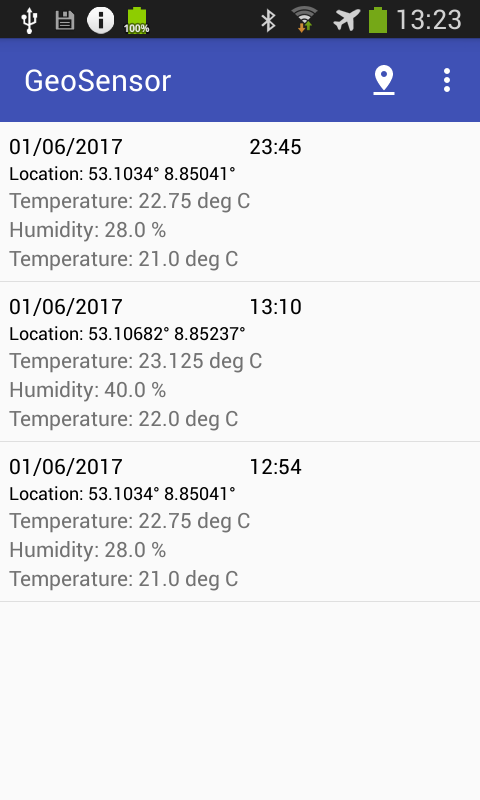
\includegraphics[width=.4\linewidth]{src/main_activity.png}
\caption{Main List View of the App}
\label{fig:main_activity}
\end{figure}

\subsubsection{Sorting}
The main list supports sorting the entries. On startup, the entries are sorted new to old by receive time. This default order was chosen as it allows to most recent and therefore probably most interesting data record to be seen on startup and also conforms to the order most social media services use for their information nowadays. There is a sorting button in the toolbar (or in the overflow menu if there is not enough space left in the toolbar) to select the sort order.

\subsection{Main Map}
\label{subs:mainmap}
Leveraging Googles Maps API (see \cite{GMapsAPI}), the app provides a map view in which every measurement is represented as a marker on the map. The map can be zoomed and rotated as a user familiar with the Google Maps app that is preinstalled on most Android devices, would expect. When a marker is tapped, an overlay window shows the measured values. The overlay can be tapped to show the details view for the respective data record. Filters work on the map the same as on the list. As the map is provided by the online Google Maps service, an internet connection is necessary to use the map view.

\begin{figure}
\centering
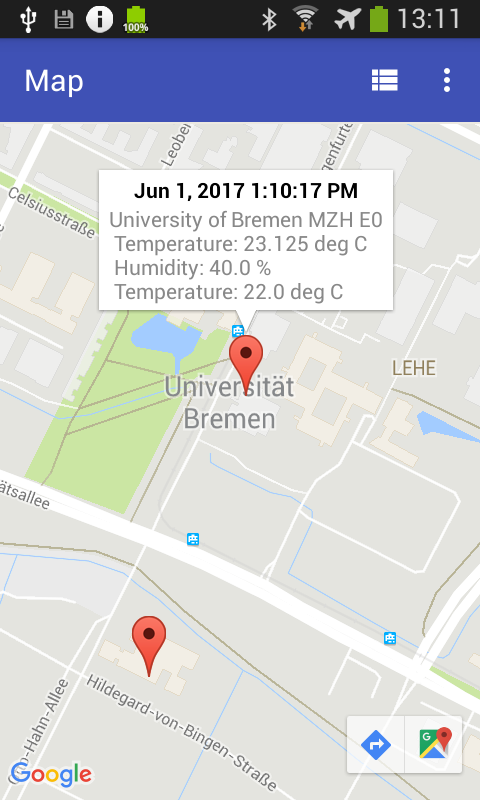
\includegraphics[width=.4\linewidth]{src/main_map.png}
\caption{Main Map View}
\label{fig:main_maps_view}
\end{figure}

\subsection{Details View}
\label{subs:details-view}
The details view is a card view (more information about the card view design pattern can be found in the Material Design Guideline \cite{Material}) showing all information available regarding a data record. It contains a card for every location associated with the data record (which might be more than one in case the transducer has a GPS receiver and the Android device location is switched on as well), a card showing all the associated locations on a map and a card for each measured sensor value.

\begin{figure}[h]
\centering
\begin{minipage}{.33\textwidth}
  \centering
  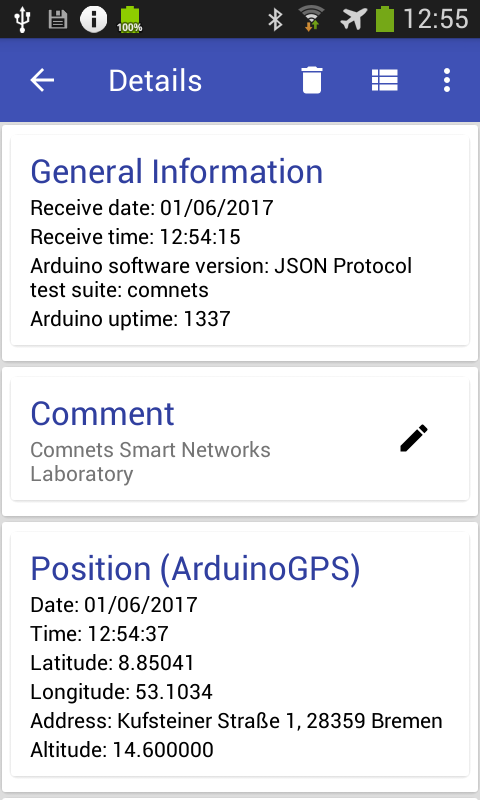
\includegraphics[width=.95\linewidth]{src/details_1.png}
\end{minipage}%
\begin{minipage}{.33\textwidth}
  \centering
  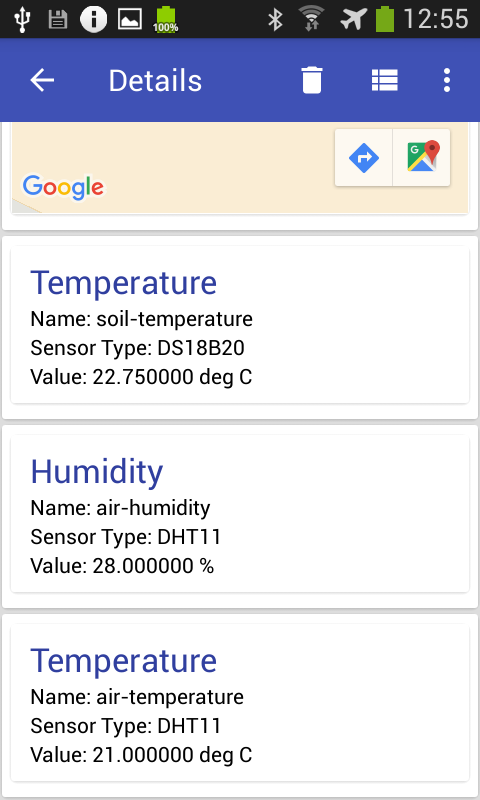
\includegraphics[width=.95\linewidth]{src/details_2.png}
\end{minipage}
\begin{minipage}{.33\textwidth}
  \centering
  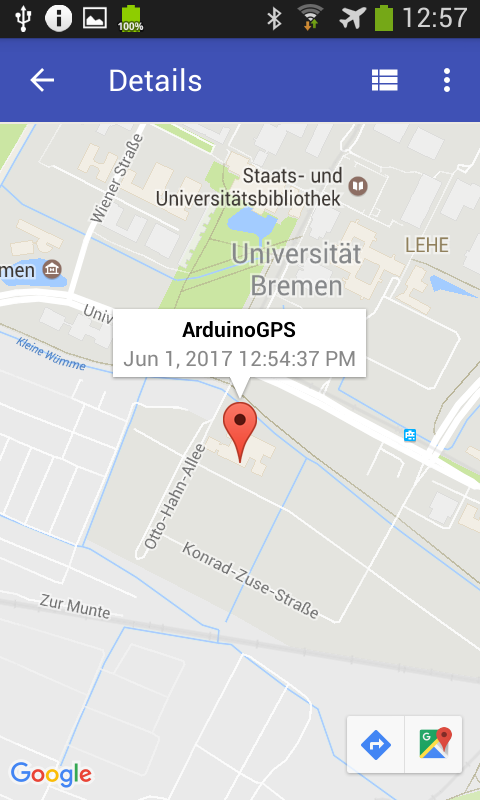
\includegraphics[width=.95\linewidth]{src/details_map.png}
\end{minipage}
  \caption{Details View}
  \label{fig:details_view}
\end{figure}

\subsubsection{General Information}
The general information card contains all the information included in a message of the protocol but not related to a sensor or the location. This includes the embedded software version deployed on the Arduino, the time when the data record was received and the uptime of the Arduino device when the message data was build.

\subsubsection{Comment}
The comment is a string that might be changed by the user. It is initially sent by the transducer device and can be modified in the app. In order to modify the comment, the user needs to touch the pencil icon on the comment card and he will be able to modify it in an alert dialog. The comment is included in the export data and therefore must not contain the field separator used in the export files. As a rule of thumb all three possible separator characters should not be included in the comment. As the export files do not specifically use an extended character set it is also advisable to use only characters contained in the ASCII-charset in the comment field.

\subsubsection{Location Data}
For each location that is associated with the data record, a separate card is shown. While all other views only show the best location available for the data record, all locations are shown in the details view. The card contains all available location information like altitude and precision if they have been included by the location provider. Data fields that are not available are not shown. If an internet connection is usable, Googles reverse geocoding API is used to provide a human readable street address for each location.

\subsubsection{Map}
As the main map view (\ref{subs:mainmap}), the details view uses Google Maps to show a map containing a marker for each location associated with the data record. For performance reasons the card only shows a static map. If the user wants to see an interactive map, they can tap the map and get an activity containg a full map. If there is no internet connection available to load the map, this card is not shown.

\subsubsection{Measured Values}
Every measured value transmitted according to the protocol (as defined in \ref{sec:protocol}) consists of five data fields which are shown in this card. All measured values have separate cards even if they have the same measurement category or are derived from the same sensor.

\subsection{Settings}
The application settings can be reached using the overflow menu in one of the activities. They are grouped into different categories (preference groups).

\subsubsection{Bluetooth Connection}
The Bluetooth connection category contains some of the most important settings for the app. 

The first setting switches the Bluetooth connection to the transducer device on or off. If this setting is on, the app will continuously hold a connection to the transducer device or be searching for a transducer device. As this requires Bluetooth, in newer Android versions the according runtime permission is requested when the Bluetooth connection is switched on. If Bluetooth is switched off in the system settings or the quick settings, the user is prompted to activate Bluetooth.

The second setting allows the user to select the Bluetooth device to which the app connects. When tapped, a list of all the paired Bluetooth devices is shown. The user should pair the Bluetooth device beforehand as programmatically coupling a device might lead to unforeseen problems (it however in general is possible). Coupling a Bluetooth device in Android is an undocumented function that can however be used acquiring a function handle using the Reflection API. The User then sees a dialog asking them to input the key needed for pairing. Under the list, a button is shown which allows the user to search for Bluetooth devices not paired yet. The devices are added to the list shown as they are found. If the user chooses a device from that list he should be shown a dialog asking him to pair the device.

The third option allows the users to choose if they want to be notified when a new data record is received. If the option is active a big text notification including the measured values is shown every time a data record is received. In order to not spam the notification area, any old notification is automatically replaced by a new one and thus at most one notification is shown.

\subsubsection{Position}
As defined in \ref{sec:location}, the app can record a position for the data records even if the transducer device does not contain a GPS module. The user has two options that can be activated in this section. The first one allows them to use a low energy method provided by Google to fix the location after a data record has been received. In slow moving applications, this approach should be sufficiently fast. The second option allows them to activate background GPS while the app is connected to the transducer. While background GPS is enabled, high accuracy positions are available as long as there is sufficient GPS signal reception. The GPS only feature might work on devices that do not provide Google libraries even though those devices are not part of the target device group for this app. The accuracy and speed if the first method is greatly improved while background GPS is activated.

\subsubsection{Data Export}
In the data export category the user can chose the decimal mark and the column separator for the export files. This is necessary as different programs have different requirements for data imports. A German version of Microsoft Excel for example needs a comma as decimal mark and a semicolon as column separator while Matlab needs a period as decimal mark and a comma as column separator. As described in (\ref{subsubs:export}) the third option allows to only export the best location available for each data record.

\subsubsection{Data}
The database section contains two options to allow basic database handling. One option lets the user chose a threshold date and cleans all older data records, the other one drops all contents of the database.

\subsubsection{Transducer Device}
In the transducer device section a message resend from the transducer device can be triggered.

\subsection{Miscellaneous Features}
\subsubsection{Automatic Database Backup}
On devices running Android 6.0 Marshmallow or newer, the app leverages the auto backup capability offered by the Android System and Google Drive. Auto Backup is a service meant to provide zero-configuration application backups. If the user uses Google Drive, the application database is regularly backed up to Google Drive. When the application is reinstalled (which would normally delete the application data on the device) the auto backup mechanism might restore the old database.

\subsubsection{Application Logo}
The application logo is a map marker in a yellow circle. It is shown in figure \ref{fig:logo}.

\begin{figure}[h]
\centering
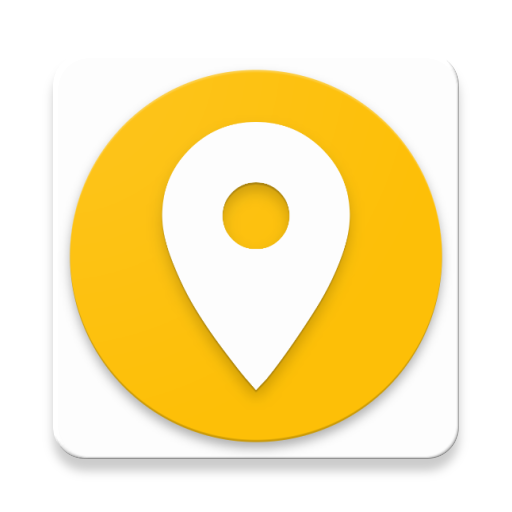
\includegraphics[width=.2\linewidth]{src/logo.png}
\caption{Application Logo}
\label{fig:logo}
\end{figure}

\subsubsection{Bluetooth Status Notification}
When the app is either searching for the selected Bluetooth device or connected to it, a notification is shown in the Android status bar. This notification enables the user to be actively aware of the state of the app even when the app is not running in the foreground. At the same time, a foreground notification gives the service a higher priority which means it is less likely to be stopped by the Android system. A tap on the notification leads to the application settings while the app is searching for the chosen device as this facilitates turning off the connection or changing the device to connect to. While the app is connected, tapping on the notification leads to the main activity and therefore to the most recent measurements received.

\begin{figure}
\centering
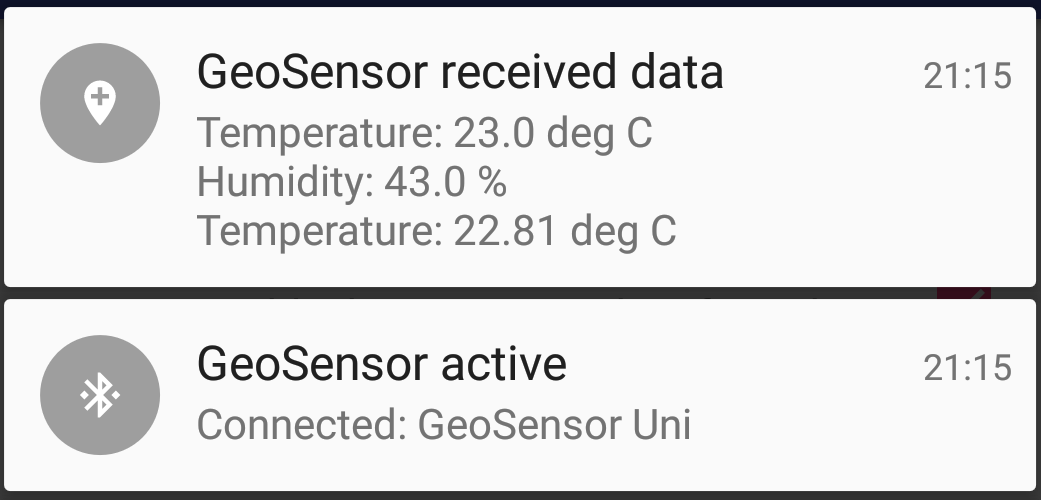
\includegraphics[width=.4\linewidth]{src/notification.png}
\caption{Notification as seen on Android 6.0 Marshmallow}
\label{fig:notification}
\end{figure}

\section{Backend}
Like most Android Apps, the app is written in the Java Programming Language (see \cite{JavaSpec}). The code was developed in Android Studio (see \cite{AndroidStudio}) and can be build using the Gradle build system included in Android studio.

\subsection{Dependencies}
Apart from the Android Platform itself (the app is built for target SDK version 25), the app does use two other libraries to provide core functionalities.

\subsubsection{Android Support Library}
The app uses the following modules of the Android Support Library (see \cite{AppCompat}) in order to provide the material design components used for all supported versions of Android:
\begin{itemize}
\item com.android.support:appcompat-v7
\item com.android.support:preference-v7
\item com.android.support:cardview-v7
\item com.android.support:design
\end{itemize}

\subsubsection{Google APIs for Android}
In addition to the Android APIs, the app uses two libraries provided by Google, which are available on Android devices equipped with the Google Play Store. 

\paragraph{Fused Location Provider API}
The Google Location Services include the Fused Location Provider API. This API offers an additional abstraction layer for the Android Location API. It combines information derived from different hardware resources into a single API that delivers the best results available at the time of the request. For example, this API might provide a WiFi-Based position when indoors and aggregate information derived from the GPS, GLONASS, Baidu and Galileo satellite navigation systems depending on which of these are available on the respective device. 

\paragraph{Google Maps API for Android}
As the app should visualize the location of the measurements on a map, the app needs a map. As including an offline map into the app would take an unreasonable or even unfeasible amount of storage space, the app needs to use online maps. On the Android platform, the most common provider for maps is Google and therefore users typically expect to see a Google Map where a map is needed. Apart from the map itself, the API includes a reverse geocoding function that can be used to retrieve a nearby human-readable street address for a given geographical location.

\subsection{Class Structure}
\subsubsection{Activities}
As most Android applications, this app is made of multiple activities. All activities in the app are derived from the GeoSensorActivity which in turn is a chile of AppCompatActivity. This allows the activities to contain a Toolbar (also from the Support Library) as action bar and follow the material style on all supported Android versions. While the toolbar used is the same in all activities, the activities show different action items in it and the selection of option items in the Toolbar is handled exclusively by the Activity showing it.

\subsubsection{Helper Classes}
The application contains helper classes for different tasks. The function of the helper classes is explained in the following subsections ordered by their role in the app.

\subsection{Bluetooth Communications}
\label{subs:bt-tech}
The Bluetooth communications are handled by a service class named BluetoothReceiverService. The service has 5 distinct states and a well-defined set of transitions that might occur between these states. The following paragraphs explain the states and the possible transitions between them. The state variable set to initialising when it is created (i.e. before the constructor and the onCreate lifecycle method are called). The service continues to run in any state until it is stopped by the framework (typically due to low memory or because the user actively closed (not just suspended) the app.

\paragraph{Initializing}
The initializing state is the first one when the service is started. During the initialising state the constructor and the onCreate lifecycle method are called by the Android framework. These methods mostly register broadcast receivers for the Bluetooth status broadcasts, some application internal broadcasts and a listener for application setting changes. After that, the service tests, if the application settings have been correctly set. If not (which should be the case only on first start), the FirstStartActivity is started in order for the user to choose the Bluetooth device to connect to. Then the service determines if the Bluetooth connection is enabled in the application settings. If it is not, it will go into the disabled state after the initialization process for the Service is finished. If the connection is enabled in the application settings, but Bluetooth is disabled, an intent asking the user to enable it is started and the state is set to \emph{Bluetooth off}. Finally if the initialization is finished, the connection is enabled and Bluetooth is available, the state is changed to \emph{searching}.

\paragraph{Bluetooth off}
The service does not do anything besides listening for broadcasts while Bluetooth is switched off. If Bluetooth is enabled by the user (often as a result of an intent asking them to do so), the service determines if the connection is enabled in the application settings and changes to the \emph{disabled} state if it is not and to the searching state if it is. 

\paragraph{Disabled}
This state is used when the Bluetooth connection is disabled in the application settings. The service continues to listen for preference changes and switches to the searching state when the correspondent setting is enabled.

\paragraph{Searching}
In the searching state the service will regularly try to connect to the transducer device chosen by the user. As waiting for a Bluetooth connection is a long-running task, the connection attempts are carried out in a different thread. As the task should not be interrupted by the system, it shows an ongoing notification and informs the Android system it runs in the foreground (i.e. it is a service the user is actively aware of). While the Bluetooth connection is searching, it retries to establish a connection about five seconds after a failed connection attempt. If the connection is established, the state is changed to connected. The other state transitions that might occur are to Bluetooth off if a broadcast is received and to disabled if the user changes the preferences.

\paragraph{Connected}
While the transducer device is connected, the service employs a thread which is constantly polling the communication channel for new bytes received. The incoming bytes are put into a string buffer and given to the parser function if the end of text (0x03) character is detected. In the connected state messages can be send to the transducer device. A state transition from the connected can occur to the Bluetooth off and disabled states for the same reason it would occur from the searching state and to the searching state if the connection is lost. A connection loss is detected through the system-wide ACL disconnected broadcast. This broadcast announces a connection loss in the link layer protocol. The ACL (asynchronous connection-less) link layer protocol typically waits 20 seconds after the last message until it considers a connection lost, under normal conditions the radio frequency communication (RFCOMM) protocol used uon top of ACL keeps the connection alive.

\subsubsection{Service Interface}
The Bluetooth stack was designed to specifically suit the requirements of the transducer device designed for this thesis, therefore only little interaction is needed. The user can use a button to trigger measurements and use the application settings to change the transducer device to connect to and deactivate the Bluetooth connection. The communications between other app components and the service uses a listener for changes in the applications shared preferences and broadcast receiver for all other communications within the app. Broadcasted intents are used for communication both towards and from the service. Other components might broadcast an intent containing the string \texttt{acquireMeasureData} if they want the service to transmit a signal requesting a measurement from the transducer and containing \texttt{resendMeasureData} if they want to trigger a resend. 

An intent is broadcasted from the service to notify other parts of the app when a new data record has been received. This intent contains the string \texttt{dataRecordReceived}.

\subsection{Data Backend}
The data backend uses a SQLite database to store the data at rest and an object-oriented approach to handle the data while the app is used. The SQLite version included in the respective Android platform is used to handle the data saved to the database which is named \emph{MeasureData.db} and saved in the applications private data directory. As the database resides in the private storage directory of the app, it is automatically backed up by the \emph{Auto Backup for Apps} technology (see \cite{Backup}) on recent Android versions. The database model closely resembles the data object model used in the app and can be found in figure \ref{fig:database}.

\begin{figure*}[h]
\centering
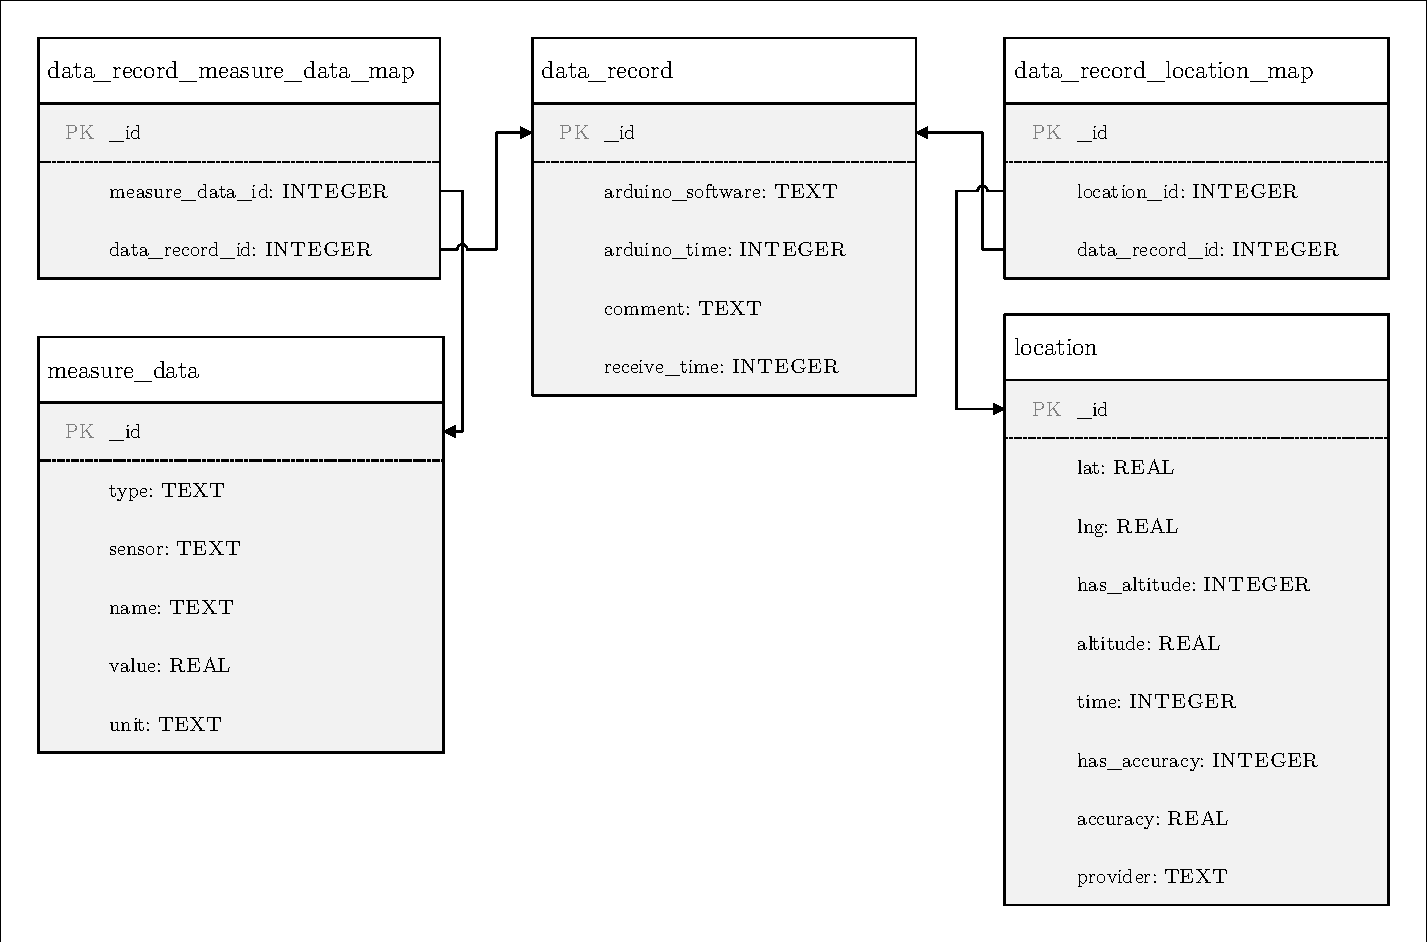
\includegraphics[width=1.0\textwidth]{src/database.pdf}
\caption{Database Model}
\label{fig:database}
\end{figure*}

All database handling in the app is done by instances of the DataLab class. The DataLab class provides all means necessary for the conversion between database data at rest and the objects used in the other parts of the app. Additionally it also includes the methods used to parse the incoming data from the JSON messages received.

\subsubsection{Data Objects}
The object-oriented data model used while the data is shown is based on the DataRecord class. For every measurement that is handled in the app a data record object is used. All data fields in a data record except the comment are immutable not only during the object lifecycle, but from the time they are first inserted into the database. The same data can be read into a DataRecord object multiple times and therefore identical copies might exist. If the comment is changed, it is immediately written into the database but other copies that exist at the same time are not affected. As a data record might include the measurements of different sensors, the sensor data for each value read from a sensor is saved in a separate object of the MeasureData class. The data record object contains a list of MeasureData objects associated with it. MeasureData objects are immutable. The data record also contains a list of Location objects including the location data derived from different sources. For reference, the information contained in the different data objects is:

\begin{itemize}
\item DataRecord
\subitem List of the associated measure data objects
\subitem List of the associated geographic locations
\subitem The time it was received (based on the Andoroid clock)
\subitem The uptime of the Arduino system when the data was sent.
\subitem The (user-editable) comment
\subitem The unique ID used in the database
\item MeasureData
\subitem The measurement category
\subitem The sensor type used
\subitem A name given for the sensor
\subitem The numerical measured value
\subitem The unit of the measurement. 
\item Location (the Location class is part of the Android framework, but only the properties mentioned here are put into the database)
\subitem Latitude
\subitem Longitude
\subitem Altitude
\subitem Time
\subitem Accuracy
\subitem The location provider used
\end{itemize}

\subsubsection{Data Parsing}
Data transmitted from the transducer device to the app is according to the protocol specification encoded in the JavaScript Object Notation (JSON) and can therefore easily be converted into Java objects. The contents of the JSON message directly correspond to the object structure used in the app. The structural JSON parsing itself is done by the \texttt{org.json} library included in the Android platform. The parsing code can be found in the DataLab class.

\subsubsection{Database Model}
As all data objects (except for the lists of other objects) contain a constant set of data fields, they can easily be represented as rows in a relational database layout. This means there is a table for DataRecord objects, one for MeasureData objects and one for Location objects. There are separate tables mapping the MeasureData and Location entries to the DataRecord objects. While adding the primary key of the DataRecord object to the Location and MeasureData tables as foreign keys, this solution is more versatile regarding future changes as it allows many-to-many relations.

\subsubsection{Filtering}
\label{subsubs:filter-tech}
Filtering by time is a feature directly derived from the database engine. As the database stores the time as an integer timestamp, both a lower and an upper limit can easily be included into the SQL-query.

\subsubsection{Sorting}
Much like filtering by time, sorting by time is a feature directly taken from the database engine.

\subsubsection{Deleting Data}
Besides the possibility to delete a single data record available in the details view, the application settings expose the option to delete old items or to drop the whole database. If the user chooses to drop the database, all tables are dropped and created from scratch again, if only old data should be deleted, the database is queried for all data records including a timestamp older than the user-chosen threshold and deletes these using the delete method for single data records which also follows the mappings in order to delete the associated location and measure data entries.

\subsection{CSV Export}
\label{subs:csv_export}
The comma separated values (CSV) export feature has been specifically designed for this app and does not use any libraries apart from the standard Java string handling. If a CSV-file should be saved, the CSVWriter generates a column layout that has enough space for all locations and measured values included in any of the data records exported. The data records to be exported are given to the CSVWriter class as a list of the DataRecord's database IDs. The CSVWriter loads all DataRecords into memory and generates a string containing all information included in the data record and formatted according to the columns generated for this export. As the export should be as versatile as possible, the user can choose their preferred decimal mark (either a dot / full stop or a comma) and value separator (comma, semicolon or tab stop). The table is then concatenated line-by-line and saved to the filesystem. On Android versions before Android 4.4 KitKat (API level 19) the file is saved to the public storage of the phone and can be opened by other apps or transferred to a computer using the USB connection. When the exported file is ready, an alert dialog is shown. On devices running Android KitKat or newer, a file provider is used to grant access to the data to a third party application handling files. When the file is ready, the user is asked to choose an app to handle the data. Typically cloud storage providers offer to take such data and save it to their clouds. For development purposes Google Drive is used as the reference cloud storage provider, but others like Microsoft OneDrive and Dropbox should work as well. A major advantage of this method is that there are no copies of the data permanently residing on the Android device as the app can delete it's copy of the data immediately after the export is completed.

\subsection{Positioning Strategies}
\label{subs:geolocalisation_strategies}
Apart from the position data provided by the transducer device, the application software enables the system to record location data provided by the Android system software. There are two different methods used for positioning which do however interact.

\subsubsection{Android GPS Location Provider}
Most Android devices contain an embedded hardware GPS receiver. If they do, a location listener can be employed to get location updates from this sensor. Typically, GPS sensors do provide a high location accuracy (between four and 20 meters for a 68 \% \/ $1~\sigma$ confidence interval) but do need good signal reception and a long startup time. As waiting a long time (often between 30 seconds and two minutes) before the location is recorded is unacceptable in most use cases, the GPS receiver must be activated before the measurements are triggered. While the Android GPS Location Provider is switched on in the application settings, the Bluetooth receiver service registers a location listener that gets regular location updates while there is a Bluetooth connection to the transducer device.

\subsubsection{Google Fused Location Provider} 
The Fused Location Provider provided by the Google Play Services on Android devices equipped with the Google Apps (which are virtually all commercially available devices outside of China) offers information derived from different sensors. While the API is similar to the one employed by the GPS location provider the fused location provider typically delivers high accuracy results much faster than the GPS location provider. In order to avoid unnecessary power consumption, the fused location provider is therefore is activated to get the location only when a data record has been received. There is a class called \texttt{DelayedLocationProvider} that is used to get the first high accuracy position when it is ready. If after 40 seconds no high accuracy location can be fixed the fused location provider is asked to provide the best location possible even if is low accuracy or outdated. 

\section{Software Quality}
While users of other platforms are often forced to use software that does not work as expected and needs workarounds to be known by the user, users of mobile platforms typically expect application software to \emph{just work}. Furthermore, the Android platform proposes a set of core app quality criteria (see \cite{CoreAppQ}) an app can be tested against. While most criteria should be met \emph{by design}, this section documents considerations about the criteria that are not completely met.

\subsection{Libraries}
The app includes and slightly outdated version of some libraries in order to support the Android API level 9. If the newest versions would be used, as of May 2017 the minimum API level would need to be elevated to 14.

\subsection{App State}
Being ready to receive data via Bluetooth even while the app is in the background is considered a core capability of the app and therefore does not violate the FN-S1 quality rule defined in the core app quality guidelines.

\subsection{Known Issues}
\subsubsection{Vector Drawables}
There is a problem using vector drawables as notification icons on versions of Android prior to 5.0 Lollipop. In these versions, other icons taken from the Android class are used.

\subsubsection{Zooming in Google Lite Maps}
The map used in the details view might in some cases exhibit strange zoom levels. This behaviour has been reviewed but no solution has been found. When the map is clicked, the larger map shown does however show normal behaviour.
